% last updated in April 2002 by Antje Endemann
% Based on CVPR 07 and LNCS, with modifications by DAF, AZ and elle, 2008 and AA, 2010, and CC, 2011; TT, 2014; AAS, 2016

\documentclass[runningheads]{llncs}
\usepackage{graphicx} \usepackage{subfigure}
\usepackage{amsmath,amssymb} % define this before the line numbering.
\usepackage{ruler}
\usepackage{color}
\usepackage[width=122mm,left=12mm,paperwidth=146mm,height=193mm,top=12mm,paperheight=217mm]{geometry}
\begin{document}
% \renewcommand\thelinenumber{\color[rgb]{0.2,0.5,0.8}\normalfont\sffamily\scriptsize\arabic{linenumber}\color[rgb]{0,0,0}}
% \renewcommand\makeLineNumber {\hss\thelinenumber\ \hspace{6mm} \rlap{\hskip\textwidth\ \hspace{6.5mm}\thelinenumber}}
% \linenumbers
\pagestyle{headings}
\mainmatter
\def\ECCV16SubNumber{***}  % Insert your submission number here

\title{Neural Style Transfer} % Replace with your title

\titlerunning{Neural Style Transfer}

\authorrunning{Neural Style Transfer}

\author{Zehua Chen, Jiaying Yang, Yiping Xie (each member contribution level is 3)}
\institute{DD2424 Deep Learning in Data Science, KTH Royal Institute of Technology}


\maketitle

\begin{abstract}
Neural style transfer is a deep neural system to synthesis a new image that obtains the high-level information of a content image yet rendered with the texture of a style image. The pre-trained convolutional neural network (CNN) VGG-19 is now frequently used in this topic, because of its powerful performance in separating and recombining content and style of arbitrary images. In addition to the ordinary neural style transfer, we also realize some further functions, including multi-style transfer and color-preserving transfer. What is more, we also try out some improvements in the calculation of loss function by adding total variation and Laplacian term into it, which help to get the output images with better quality.
\keywords{Style Transfer,  convolutional neural network, VGG-19, Laplacian loss}
\end{abstract}


\section{Introduction}
We have upload all of our code in this project on Github\footnote{https://github.com/Chen-Z-H/Neural-Style-Transfer-based-on-CNN}. 

Neural style transfer (NST) is a technique to generate new image that can replicate the content of one input image, but combined the style of another one. This technique can be used into changing an ordinary photography into artistic style, by giving an input of an arbitrary art work. The work of Gatys \textit{et al.}\cite{GatysLeon2016ANAo} first demonstrated the power of Convolutional Neural Networks (CNN) in neural style transfer.

In this project we first replicate the experiment done by Gatys \textit{et al.} to realize the neural style transfer. Their used Gram matrix to realize the reconstruction of image style, which indicates the correlations
between filter responses in different layers of a pre-trained CNN
classification network, namely VGG-19.

Then we realize some more functions based on the theory of neural style transfer, including multi-style transfer and color preserving transfer. Multi-style transfer can transfer the combination of several style into the content image , while color preserving transfer can keep the original color of the content image unchanged after transfer.

Finally, we made some further improvements to the calculation of loss function to improve the quality of the generated image. We add the total variation regularization term to the loss function in order to improve the smoothness of the output image. Moreover, we add a Laplacian loss term to the total loss function in order to reduce the artifacts and distortions of the generated image by taking the pixel space into account.





\section{Background}
After Gatys \textit{et al.} proposed to use CNN to render a content image in the style of famous artworks, numerous studies followed up to either extend or improve the algorithm. 
The NST algorithm can be seen as the combination of visual texture modelling (and synthesis) and image reconstruction. 

Based on how the visual texture is modeled, there are mainly two distinct approaches: Parametric Texture Modelling and Non-parametric Texture Modelling. 

The parametric visual texture approach Gatys \textit{et al.}\cite{GatysLeon2016ANAo} proposed is to design a Gram matrix, which calculates the correlations between the CNN filter responses in different layers of VGG network, to measure the second-order statistics of the filter responses in the CNN domain. 
This Gram-based texture representation in the CNN domain effectively models a variety of natural and non-natural textures.

Another visual texture modelling method is non-parametric, most of which is based on Markov Random Fields (MRFs) model. This model assumes that each pixel in a texture image is fully characterised by its spatial neighborhood. Wei and Levoy\cite{LiChuan2016CMRF} proposed an approach to synthesis each pixel by searching a fixed neighborhood in the texture example image. One of the critical limitation of MRFs is that estimating the distribution of image patches from the example data is difficult and another limitation MRFs suffer from is sometimes local image statistics have a hard time fully capturing the texture of the complex image. However, this patch-level matching algorithm can preserve fine structure and arrangement better, which means it can work remarkably for photo-realistic styles. 

Based on the speed of image reconstruction, there are also two approaches: Slow Image Reconstruction and Fast Image Reconstruction.

The idea based on Slow Image Reconstruction is to model and extract the content and style information and then recombine them as the target representation, which can be updated iteratively until it matches the desired CNN feature distribution. This optimising process can be very time-consuming and inefficient thus lots of researchers proposed an approach to leave the huge computation burden at the training stage: training a feed-forward neural network in advance so that the reconstruction process can be done simply with a forward pass at the test stage\cite{JohsonJustin2016PLfR}\cite{UlyanovDmitry2016TNFS}. These Fast NST algorithms are able to generate stylised images in real-time, even though in terms of minimising the loss function, they are not good as Slow NST algorithm\cite{jing2017neural}. Depending on the number of styles one model can produce, Fast NST algorithms can be divided into Per-Style-Per-Model\cite{JohsonJustin2016PLfR}\cite{UlyanovDmitry2016TNFS}, Multiple-Style-Per-Model\cite{ZhangHang2017MGNf}\cite{DumoulinVincent2016ALRF}, and Arbitrary-Style-Per-Model\cite{ChenTianQi2016FPST}\cite{GhiasiGolnaz2017Etso}.  
\section{Approach}
\label{sec:theory}
\subsection{Theory}

%\subsubsection{Content Representation}
The theory below mainly follows Gatys \textit{et al.}'s work.

\begin{figure}[h!]
    \centering
    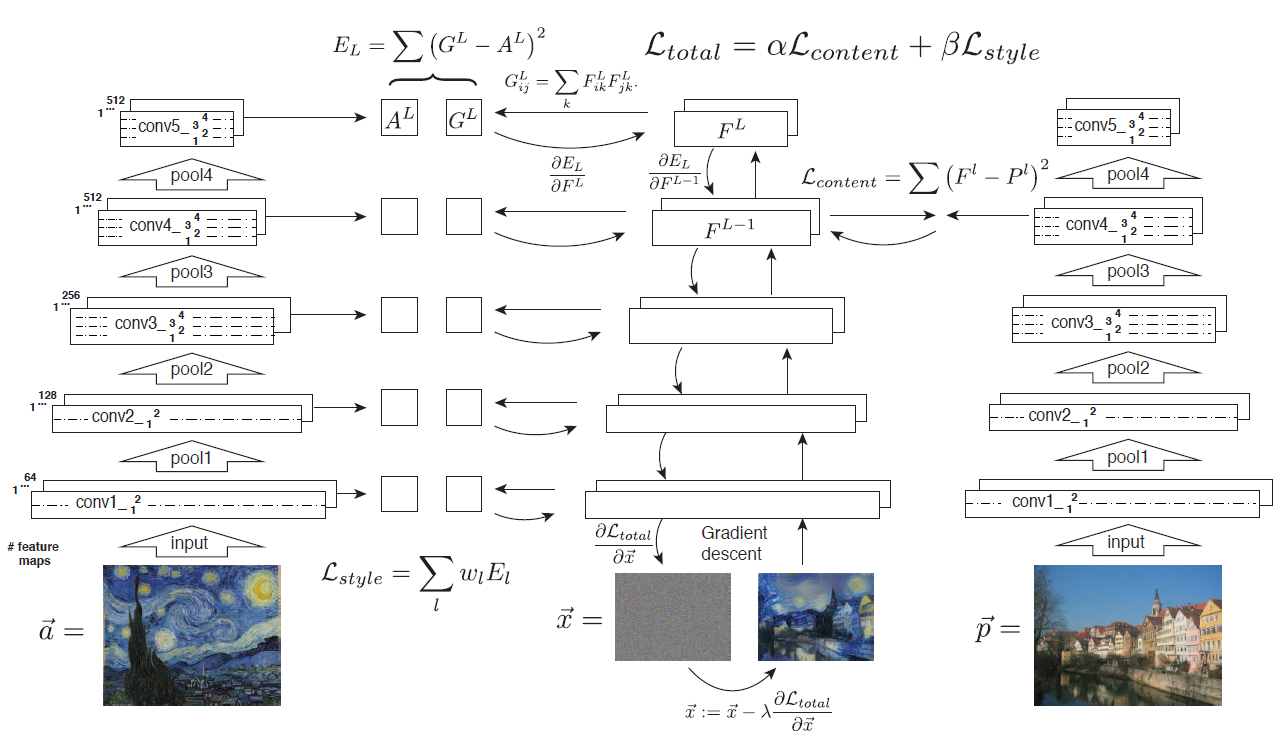
\includegraphics[scale=.4]{neural_style_transfer/img/transfer_algorithm.png}
    \caption{Basic style transfer algorithm}
    \label{fig:algorithm}
\end{figure}

In the VGG network, each layer represents a filter response to the image. Given a source image $\vec{x}$, a layer $l$ with $N_l$ distinct filters has $N_l$ feature maps each with the size of $M_l$, where $M_l$ equals to the multiplication of the feature map's height and width. Thus the response for layer $l$ can be represented as a matrix $F^l \in \mathcal{R}^{N_l \times M_l}$ where $F^l_{ij}$ is the activation of the $i_{th}$ filter at the position $j$ in layer $l$.
Assume $\vec{p}$ and $\vec{x}$ to be the original content image and the generated image respectively, and $F^l$ and $P^l$ to be the respective feature representations in layer $l$. Then the content loss can be described as squared-error loss between these two representations:
\begin{align}
    L_{content}(\vec{p},\vec{x},l)=\frac{1}{2}\sum_{i,j}(F_{ij}^{l}-P_{ij}^{l})^{2}
\end{align}

Here a parametric texture modelling is used to capture the visual texture information of the input style image. This feature can be calculated as the correlations between the different filter responses in ant layer of the VGG network, given in the format of Gram matrix:
\begin{align}
    G_{ij}^{l}=\sum_{k}F_{ik}^{l}F_{jk}^{l}
\end{align}

Assume $\vec{a}$ and $\vec{x}$ to be the original style image and the generated image respectively, and $A^l$ and $G^l$ to be the respective style representations in layer $l$.
The style loss at each layer is given by:
\begin{align}
    E_{l}=\frac{1}{4N_{l}^{2}M_{l}^{2}}\sum_{i,j}(G_{ij}^{l}-A_{ij}^{l})^{2}
\end{align}

The total style loss is the combination of losses at different layers:
\begin{align}
    L_{style}(\vec{a},\vec{x})=\sum_{l=0}^{L}w_{l}E_{l}
\end{align}

Our aim is minimizing the distance of the synthetic image from the content representation as well as the style representation given by the formulas above. Thus we combine the style loss and content loss in following way:
\begin{align}
    L_{total}(\vec{p},\vec{a},\vec{x})=\alpha L_{content}(\vec{p},\vec{x})+\beta L_{style}(\vec{a},\vec{x})
    \label{eq:loss}
\end{align}
\subsection{Further Functions}

\subsubsection{Multi-style Transfer}
We can intuitively understand that the style transfer algorithm mentioned above is actually a optimization strategy that balancing the loss between multiple images. Then it is easy to come to an idea that if we balance the losses between multiple styles, we can combine the styles of several art works to generate the image. This can be achieved by modifying the formula as below:
\begin{align}
    L_{multi}=\sum_{i=1}^{n}w_{i}L_{style}(\vec{x},\vec{p}_{i})
\end{align}
where ${p_{1}, p_{2},.., p_{n}}$ is a series of style images and $w_i$ is the weight of style loss of each image. In this paper we perform the experiments of blending two distinct painting styles but we can also extend it to a arbitrary number of styles. By changing the weights of style losses we can adjust the effect each style image poses on the final generated image.

\subsubsection{Color Preserving Style Transfer}
When using the traditional algorithm to transform an content image to have the style of another given style image, we always face the shortcoming that the color of the content image is also changed. %(给个例子)
The unexpected altering of color is what we hope to avoid. Thus we improve the algorithm in order to realize the function of Color Preserving Style Transfer.

As is shown in the article\cite{gatys2016preserving}, at present there are two main methods to realize the function of color preserving, which are Color Histogram Matching and Luminance-only Transfer. We choose to use Luminance-only transfer, because compared to the first method, it can preserve the colors of the content image better.

Luminance-only transfer is realized by doing the style transfer only in the luminance channel. We first transfer the content image and style image  from RGB space into YUV space. In YUV space, the Y channel stands for the luminance information, while the U and V channels represents the color information. In order to preserve the color information of the content image and only change its luminance information, we should extract the Y channel from the style image, and the U and V channels from the content image. Finally the extracted three channels are regrouped to produce our final output image. This process is shown in Fig.\ref{fig:yuv}.

\begin{figure}[h!]
    \centering
    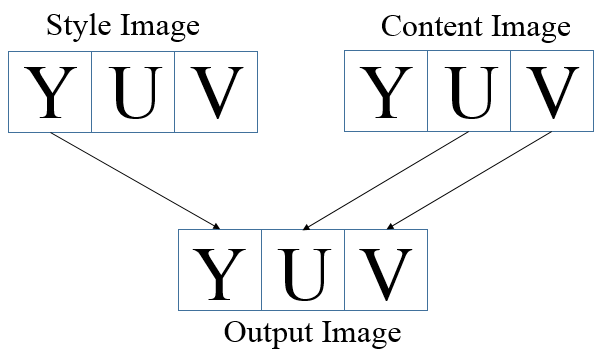
\includegraphics[scale=.4]{YUV.PNG}
    \caption{Luminance-only Transfer}
    \label{fig:yuv}
\end{figure}

In order to improve the performance of Luminance-only Transfer further, we transform the luminance of the style image $L_S$  to have the same first and second order statistics as the content image $L_C$ as below: 
\begin{align}
    L_{S^{'}}=\frac{\sigma_{C}}{\sigma_{S}}(L_{S}-\mu_{S})+\mu_{C}
\end{align}
where $L_S$ and $L_C$ are the luminance information of the style and content images; $\mu_S$ and $\mu_C$ are the mean luminances
of the two images; and $\sigma_S$ and $\sigma_C$ are their standard deviations.
\subsection{Total Variation Regularization} When calculating the total loss, in addition to the content loss and style mentioned in Equation 5 , we can also add a  total variation regularization term to the total loss $L_{TV}$\cite{JohsonJustin2016PLfR}, which can help encourage spatial smoothness in the final output image. 

The total variation is the sum of the absolute differences for neighboring pixel-values in the input images, which measures how much noise is in the images. After adding the total variation into the calculation of loss function, it can help suppress noise in the content image. The calculation of total variation loss $L_{TV}$ is calculated by using the Tensorflow function $tf.image.total\_variation$.

The calculation of loss is updated as below after this improvement:
\begin{align}
    L_{total}(\vec{p},\vec{a},\vec{x})=\alpha L_{content}(\vec{p},\vec{x})+\beta L_{style}(\vec{a},\vec{x})+\theta L_{TV}(\vec{p})
\end{align}
where $\theta$ is a constant parameter controlling the strength of the total variation regularization.
\subsection{Laplacian-Steered Neural Style Transfer}
In the algorithm mentioned above, the content loss is computed in the CNN feature space so that the synthetic image is semantically similar to the content image. However, the CNN features are high-level representations that mainly capture the semantic information, thus inevitably leading to lose some low-level features of the image, e.g. texture, colors and basic structures. 
The synthetic image will usually have some irregular artifacts and unsatisfied distortions\cite{jing2017neural}. 

To reduce the artifacts and better preserve the detailed structures of the content image, a new term named Laplacian Loss is added in the loss function\cite{LiShaohua2017LNST} by measuring the squared Euclidean distance between the Laplacian operator response of the content image and the synthetic image. 

Given an image $\vec{x}$ the Laplacian filter response $D(\vec{x})$ is computed by applying the two dimensional discrete Laplacian Operator $D$ to the image.
\begin{equation}
    D=\begin{bmatrix}
0 & -1 & 0\\ 
-1 & 4 & -1\\ 
0 & -1 & 0
\end{bmatrix}
\end{equation}
Given the content image $\vec{p}$ and the synthetic image $\vec{x}$, the Laplacian loss $L_{lap}$ is defined as 
\begin{equation}
    L_{lap}(\vec{p},\vec{x}) = \sum_{ij}[D(\vec{p})-D(\vec{x})]_{ij}^2
\end{equation}
Thus the total loss is defined as:
\begin{align}
    L_{total}(\vec{p},\vec{a},\vec{x})=\alpha L_{content}(\vec{p},\vec{x})+\beta L_{style}(\vec{a},\vec{x})+\gamma L_{lap}(\vec{p},\vec{x})
\end{align}
where $\gamma$ is a tunable parameter controlling the strength of the Laplacaian Loss constraint.

There are several practical details during the calculation of the Laplacian loss\cite{LiShaohua2017LNST} that can be addressed as below.

% \textbf{Laplacians on RGB channels}\quad
\subsubsection{Laplacians on RGB channels}
Since the input image $\vec{x}$ has RGB channels, the Laplacians should contain the result on each channels separately. Regardless the sign, the Laplacian operator can detect the edge when there is a huge magnitude in any of the three channels, so the theoretical Laplacian $D(\vec{x})$ should be calculated as the sum of absolute values of theses three Laplacians:
\begin{align}
    D(\vec{x}) = \Vert D(\vec{x}^R)\Vert +\Vert D(\vec{x}^G)\Vert +\Vert D(\vec{x}^B)\Vert 
\end{align}
Li, Shaohua \textit{et al.}\cite{LiShaohua2017LNST} proposed to approximate the theoretical result using simple summation of the three Laplacians:
\begin{align}
    D(\vec{x}) =  D(\vec{x}^R)+D(\vec{x}^G)+ D(\vec{x}^B)
\end{align}
Using this approximation, Li, Shaohua \textit{et al.} claimed that they have not observed any quality degradation of the synthetic image.

% \textbf{Smoothing with a polling layer}\quad
\subsubsection{Smoothing with a pooling layer}
The Laplacian filter is very sensitive to noise so smoothing the image with an average pooling layer before the Laplacian filter can better preserve the actual detailed structure of the content image. Besides, we can save the memory to $1/p^2$ by applying a $p\times p$ pooling layer overhead of the Laplacian loss. The size $p$ is also a parameter that can be fine-tuned in order to get a better synthetic image. 

% \textbf{Combining Multiple Laplacians}\quad
\subsubsection{Combining Multiple Laplacians}
With a kernel in bigger size, the pooling layer can squeeze a bigger area into a pixel. With a Laplacian filter overhead of the such pooling layer can preserve the structures in a wider region. Hence, it is a great idea to combine multiple Laplacians with different sizes of the Laplacian filter into the Laplacian loss, which may capture the structures in different scales. The Laplacian loss can be revised as:
\begin{align}
    L_{total}(\vec{p},\vec{a},\vec{x})=\alpha L_{content}(\vec{p},\vec{x})+\beta L_{style}(\vec{a},\vec{x})+\sum_{k} \gamma_{k} L_{lap,k}(\vec{p},\vec{x})
\end{align}
where $L_{lap,k}$ is the Laplacians overhead of a pooling layer with size $p_k \times p_k$ and $\gamma_k$ is the corresponding wight.

\section{Results}
\subsection{Tuning the Content/Style Ratio and Picking Layers}
The content image we used in this part is the photography of Stockholm, while the style image is the Chinese painting  named "Dwelling in the Fuchun Mountains" by Gongwang Huang, as is shown in Fig.\ref{fig:sto} and Fig.\ref{fig:fuchun}.
\begin{figure}[htbp]
\centering
\begin{minipage}[t]{0.48\textwidth}
\centering
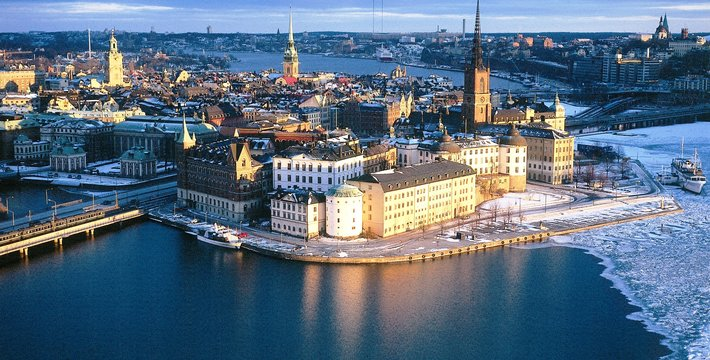
\includegraphics[width=6cm]{neural_style_transfer/img/fuchunshan_Stockholm/stockholm1.jpg}
\caption{Content Image}
\label{fig:sto}
\end{minipage}
\begin{minipage}[t]{0.48\textwidth}
\centering
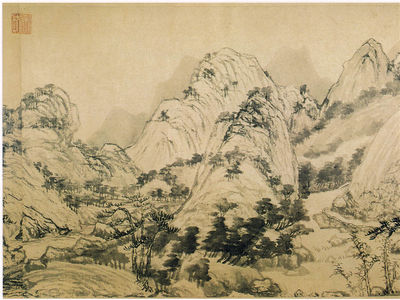
\includegraphics[width=2.5cm]{neural_style_transfer/img/fuchunshan_Stockholm/fuchunshanjutu.jpg}
\caption{Style Image}
\label{fig:fuchun}
\end{minipage}
\end{figure}

As is shown in Equation 5, there are two parameters $\alpha$ and $\beta$ in the loss function controlling the strength of the content image and style image. Their ratio $\alpha/\beta$ reflects the trade-off between the content and style information. When the content/style ratio $\alpha/\beta$ is larger, the output image remain more information from the content image, but with a less noticeable style. However, when the content/style ratio $\alpha/\beta$ is smaller, the output information will contain more style information, but less content information.

Moreover, picking different layers of the VGG-19 network will also has an influence on the output image performance. In the VGG network, the deeper layer represents more high-level information of the image, which indicates losing more low-level detailed information. As we can notice in Fig.\ref{fig:sto-fuchun}, the detailed structures, for example the edges of the buildings, can be preserved less and less as the picking layer for content image goes deep.

The output images with different content/style ratio $\alpha/\beta$ and different picked layers can be shown in Fig.\ref{fig:sto-fuchun}.
\begin{figure}[h]
\centering
\subfigure[conv1-2]{
\begin{minipage}[b]{0.15\textwidth}
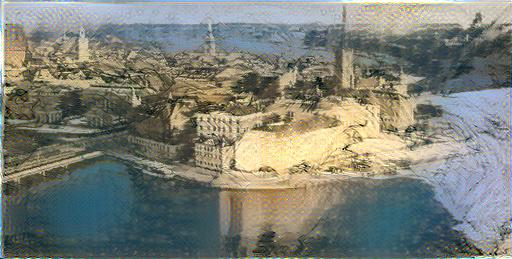
\includegraphics[width=1.1\textwidth]{neural_style_transfer/img/fu_stockholm_output/fu_stockholm_conv1-2_1e-1.jpg} \\
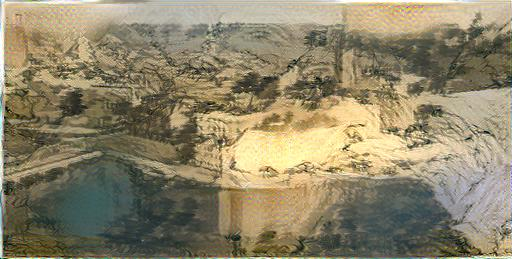
\includegraphics[width=1.1\textwidth]{neural_style_transfer/img/fu_stockholm_output/fu_stockholm_conv1-2_1e-2.jpg} \\
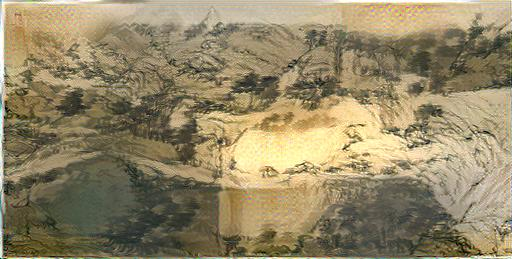
\includegraphics[width=1.1\textwidth]{neural_style_transfer/img/fu_stockholm_output/fu_stockholm_conv1-2_1e-3.jpg} \\
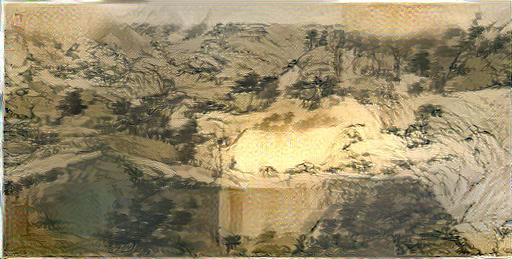
\includegraphics[width=1.1\textwidth]{neural_style_transfer/img/fu_stockholm_output/fu_stockholm_conv1-2_1e-4.jpg}
\end{minipage}
}
\subfigure[conv2-2]{
\begin{minipage}[b]{0.15\textwidth}
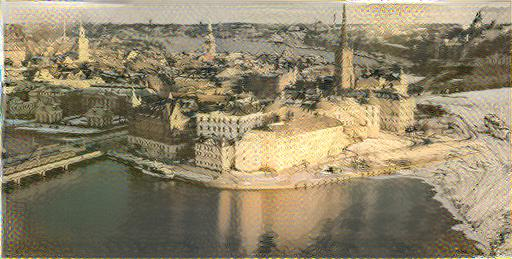
\includegraphics[width=1.1\textwidth]{neural_style_transfer/img/fu_stockholm_output/fu_stockholm_conv2-2_1e-1.jpg} \\
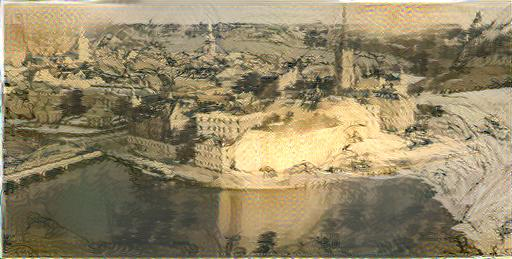
\includegraphics[width=1.1\textwidth]{neural_style_transfer/img/fu_stockholm_output/fu_stockholm_conv2-2_1e-2.jpg} \\
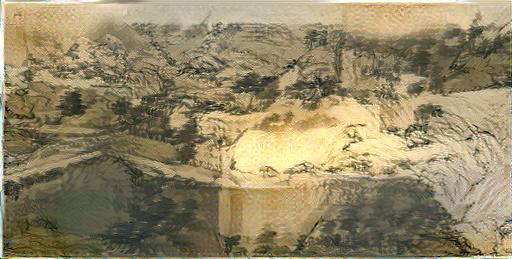
\includegraphics[width=1.1\textwidth]{neural_style_transfer/img/fu_stockholm_output/fu_stockholm_conv2-2_1e-3.jpg} \\
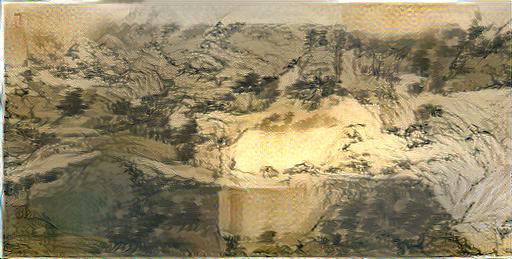
\includegraphics[width=1.1\textwidth]{neural_style_transfer/img/fu_stockholm_output/fu_stockholm_conv2-2_1e-4.jpg}
\end{minipage}
}
% \hspace{0.001in}
\subfigure[conv3-2]{
\begin{minipage}[b]{0.15\textwidth}
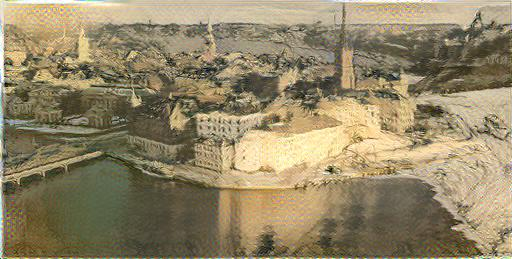
\includegraphics[width=1.1\textwidth]{neural_style_transfer/img/fu_stockholm_output/fu_stockholm_conv3-2_1e-1.jpg} \\
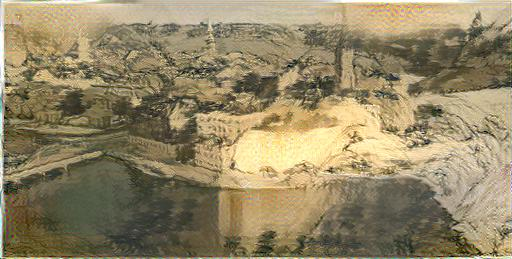
\includegraphics[width=1.1\textwidth]{neural_style_transfer/img/fu_stockholm_output/fu_stockholm_conv3-2_1e-2.jpg} \\
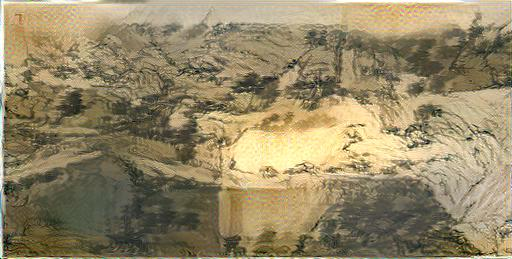
\includegraphics[width=1.1\textwidth]{neural_style_transfer/img/fu_stockholm_output/fu_stockholm_conv3-2_1e-3.jpg} \\
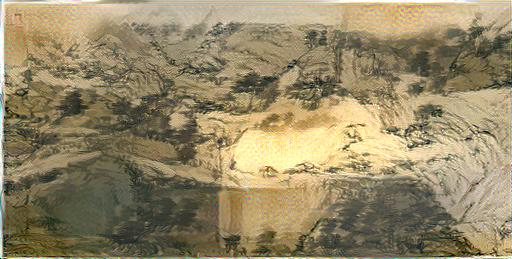
\includegraphics[width=1.1\textwidth]{neural_style_transfer/img/fu_stockholm_output/fu_stockholm_conv3-2_1e-4.jpg}
\end{minipage}
}
\subfigure[conv4-2]{
\begin{minipage}[b]{0.15\textwidth}
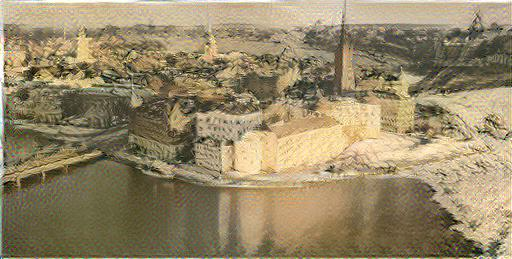
\includegraphics[width=1.1\textwidth]{neural_style_transfer/img/fu_stockholm_output/fu_stockholm_conv4-2_1e-1.jpg} \\
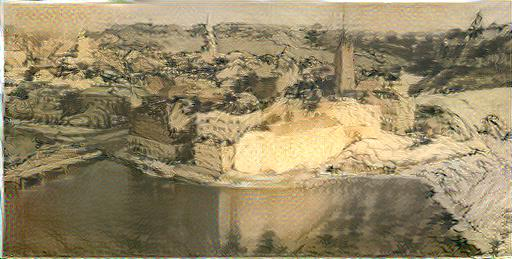
\includegraphics[width=1.1\textwidth]{neural_style_transfer/img/fu_stockholm_output/fu_stockholm_conv4-2_1e-2.jpg} \\
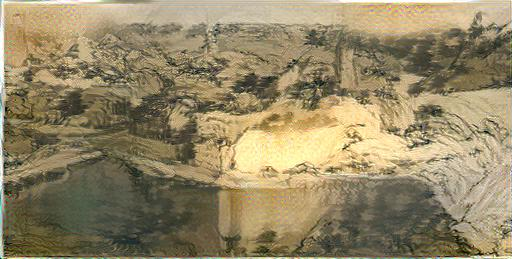
\includegraphics[width=1.1\textwidth]{neural_style_transfer/img/fu_stockholm_output/fu_stockholm_conv4-2_1e-3.jpg} \\
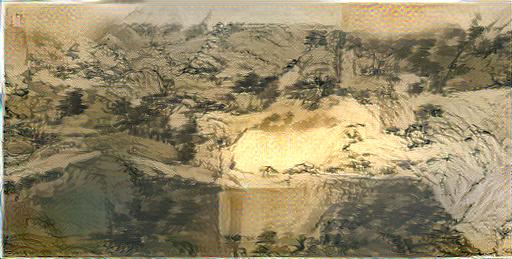
\includegraphics[width=1.1\textwidth]{neural_style_transfer/img/fu_stockholm_output/fu_stockholm_conv4-2_1e-4.jpg}
\end{minipage}
}
\subfigure[conv5-2]{
\begin{minipage}[b]{0.15\textwidth}
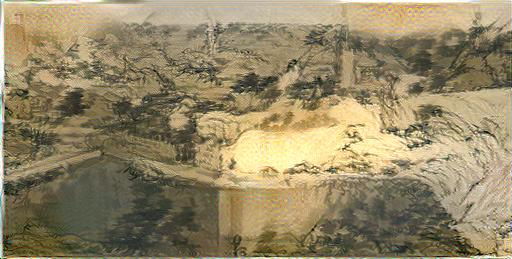
\includegraphics[width=1.1\textwidth]{neural_style_transfer/img/fu_stockholm_output/fu_stockholm_conv5-2_1e-1.jpg} \\
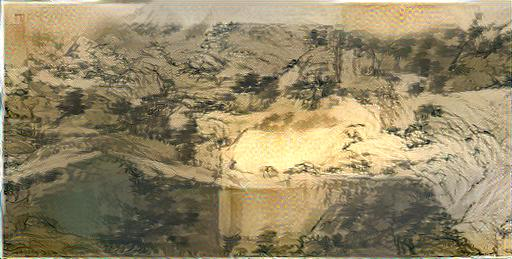
\includegraphics[width=1.1\textwidth]{neural_style_transfer/img/fu_stockholm_output/fu_stockholm_conv5-2_1e-2.jpg} \\
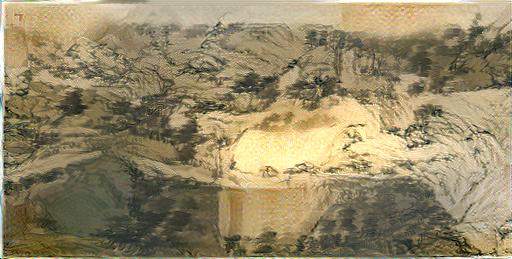
\includegraphics[width=1.1\textwidth]{neural_style_transfer/img/fu_stockholm_output/fu_stockholm_conv5-2_1e-3.jpg} \\
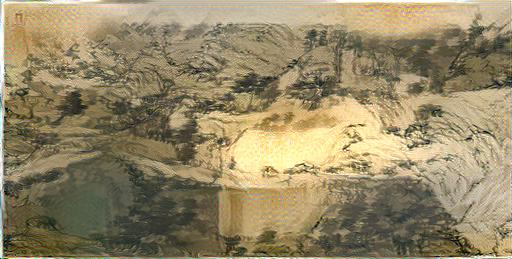
\includegraphics[width=1.1\textwidth]{neural_style_transfer/img/fu_stockholm_output/fu_stockholm_conv5-2_1e-4.jpg}
\end{minipage}
}
\caption{Reconstruction capability of different content\/style ratios $\alpha/\beta$ and representation at different layers, the $\alpha/\beta$ from top to bottom is $10^{-1}, 10^{-2}, 10^{-3}, 10^{-4}$ respectively}
\label{fig:sto-fuchun}
\end{figure}




\subsection{Multi-style Transfer}
In this part, we try out blending between the Kandinsky and the Starry Night, as well as blending between the Seated Nude and the Scream, into our chosen content image Tubingen. As we can see from the Fig.\ref{fig:multi}, the generated images contains both styles of the above style images. Depending on the loss weights, the two styles in the same image can have different contributions. An interesting observation is that, each style tends to occupy a certain part in the image.
\begin{figure}[h!]
\centering
\subfigure[Style1]{
\begin{minipage}[b]{0.15\textwidth}
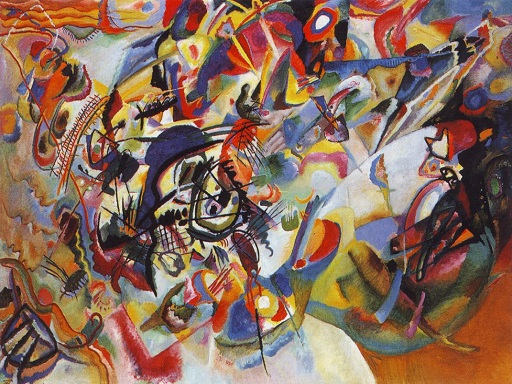
\includegraphics[width=1\textwidth]{neural_style_transfer/img/styles/kandinsky.jpg} \\
\centering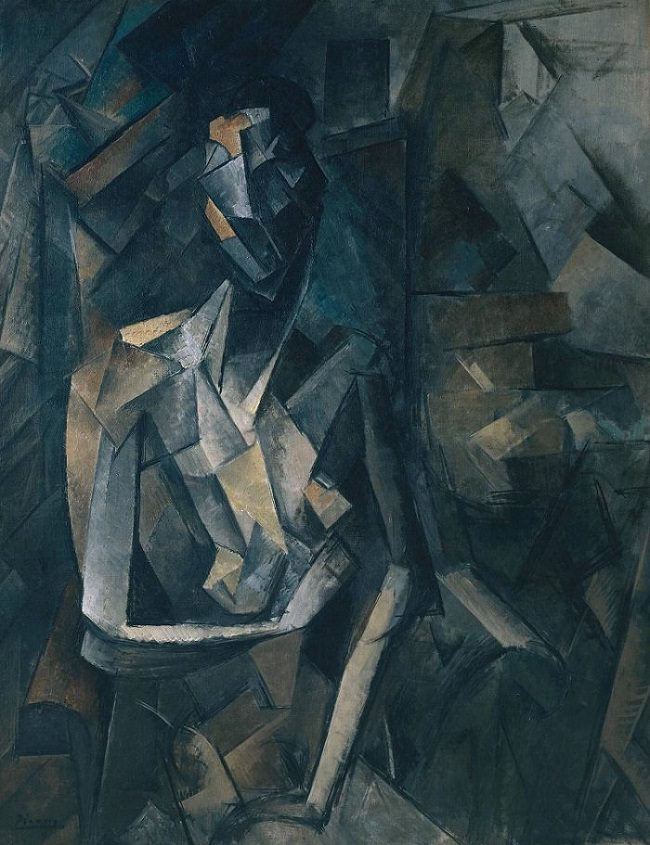
\includegraphics[width=1\textwidth]{neural_style_transfer/img/styles/seated-nude.jpg}
\end{minipage}
}
\subfigure[80\% / 20\%]{
\begin{minipage}[b]{0.15\textwidth}
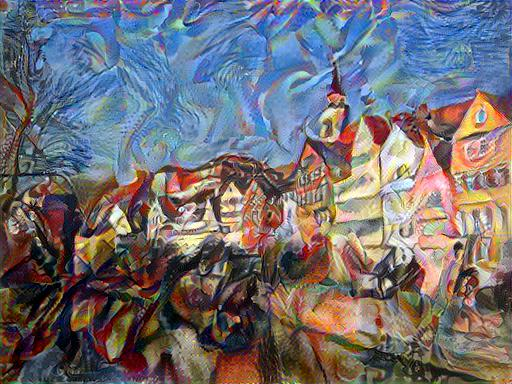
\includegraphics[width=1\textwidth]{neural_style_transfer/img/05_multi_style_output/multi_styles_0-2.jpg} \\
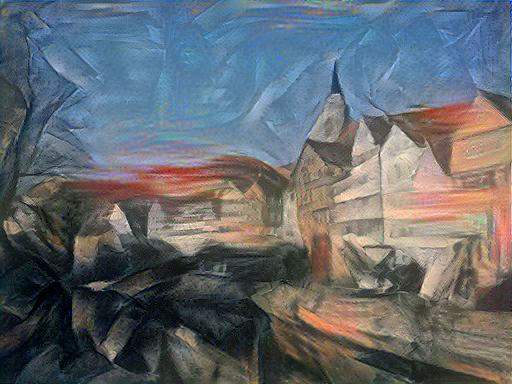
\includegraphics[width=1\textwidth]{neural_style_transfer/img/05_multi_style_output/multi_styles1_0-2.jpg}
\end{minipage}
}
\subfigure[50\% / 50\%]{
\begin{minipage}[b]{0.15\textwidth}
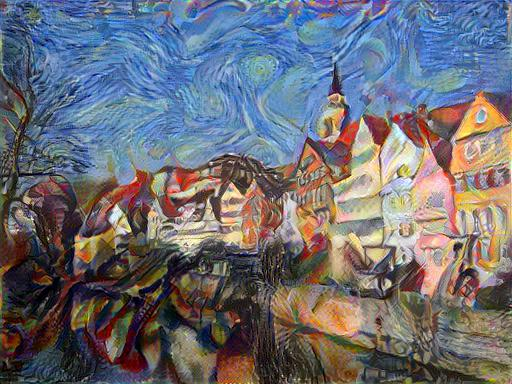
\includegraphics[width=1\textwidth]{neural_style_transfer/img/05_multi_style_output/multi_styles_0-5.jpg} \\
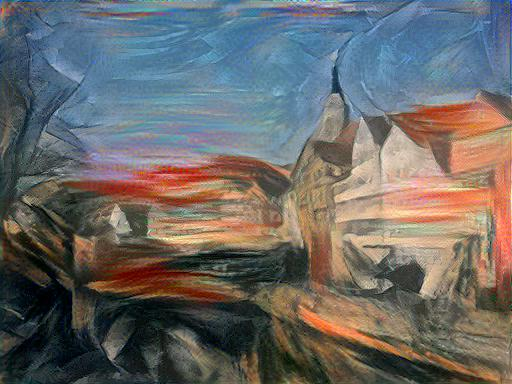
\includegraphics[width=1\textwidth]{neural_style_transfer/img/05_multi_style_output/multi_styles1_0-5.jpg}
\end{minipage}
}
\subfigure[20\% / 80\%]{
\begin{minipage}[b]{0.15\textwidth}
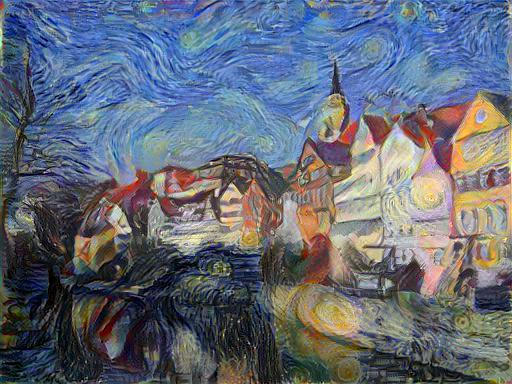
\includegraphics[width=1\textwidth]{neural_style_transfer/img/05_multi_style_output/multi_styles_0-8.jpg} \\
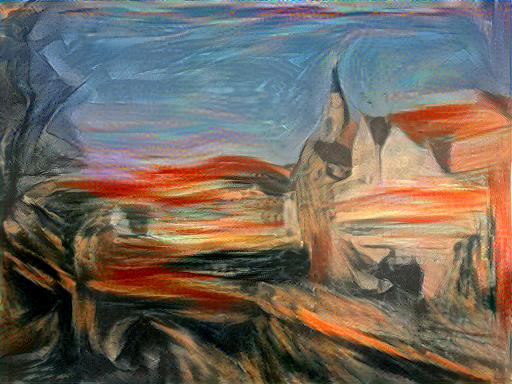
\includegraphics[width=1\textwidth]{neural_style_transfer/img/05_multi_style_output/multi_styles1_0-8.jpg}
\end{minipage}
}
\subfigure[Style2]{
\begin{minipage}[b]{0.15\textwidth}
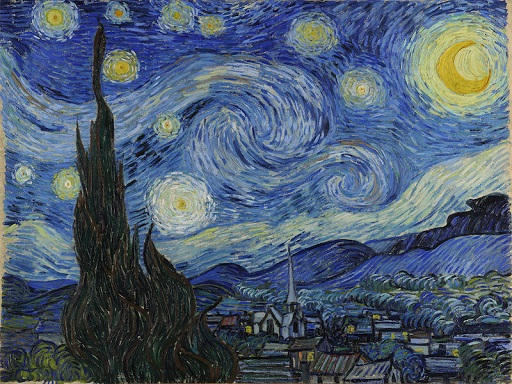
\includegraphics[width=1\textwidth]{neural_style_transfer/img/styles/starry-night.jpg} \\
\centering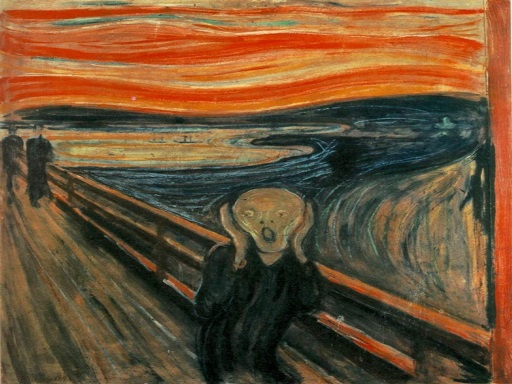
\includegraphics[width=1\textwidth]{neural_style_transfer/img/styles/the_scream.jpg}
\end{minipage}
}
\caption{Results of Multi-style transfer. By setting the weights of style losses, we can control the effects that each style image has on the synthetic image.}
\label{fig:multi}
\end{figure}

\subsection{Color Preserving Style Transfer}
In this part we choose the Tubingen as the content image and the Starry Night as the style image.

% \begin{figure}[h]
% \centering
% \subfigure[content]{
% \begin{minipage}[b]{0.4\textwidth}
% 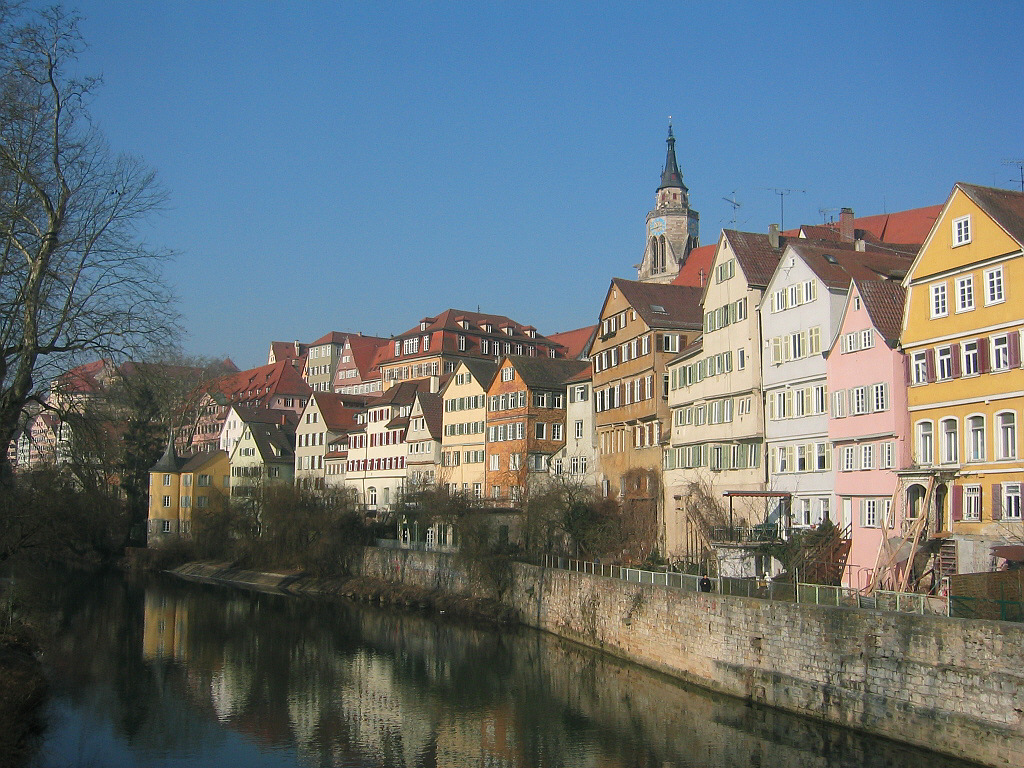
\includegraphics[width=1\textwidth]{neural_style_transfer/img/content/05.jpg} \\
% \end{minipage}
% }
% \subfigure[style]{
% \begin{minipage}[b]{0.4\textwidth}
% 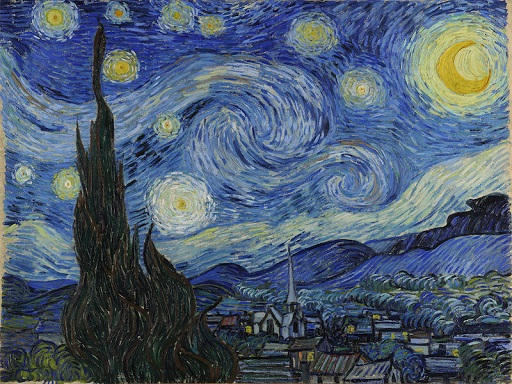
\includegraphics[width=1\textwidth]{neural_style_transfer/img/styles/starry-night.jpg} \\
% \end{minipage}
% }
% \caption{Laplace-Steered Neural Style Transfer}
% \label{fig:preserve}
% \end{figure}
The luminance-only method for color preserving style transfer works very well according to the result of our experiments. Fig.\ref{fig:preserve} is the comparison of the ordinary neural style transfer and color preserving style transfer with the same content image and style image.

We can easily find out that after the ordinary neural style transfer, the color of output image is dark blue, because of the influence of the style image. However, color preserving style transfer can keep the output image to have similar color with the content image.

\begin{figure}[h!]
\centering
\subfigure{
\begin{minipage}[b]{0.4\textwidth}
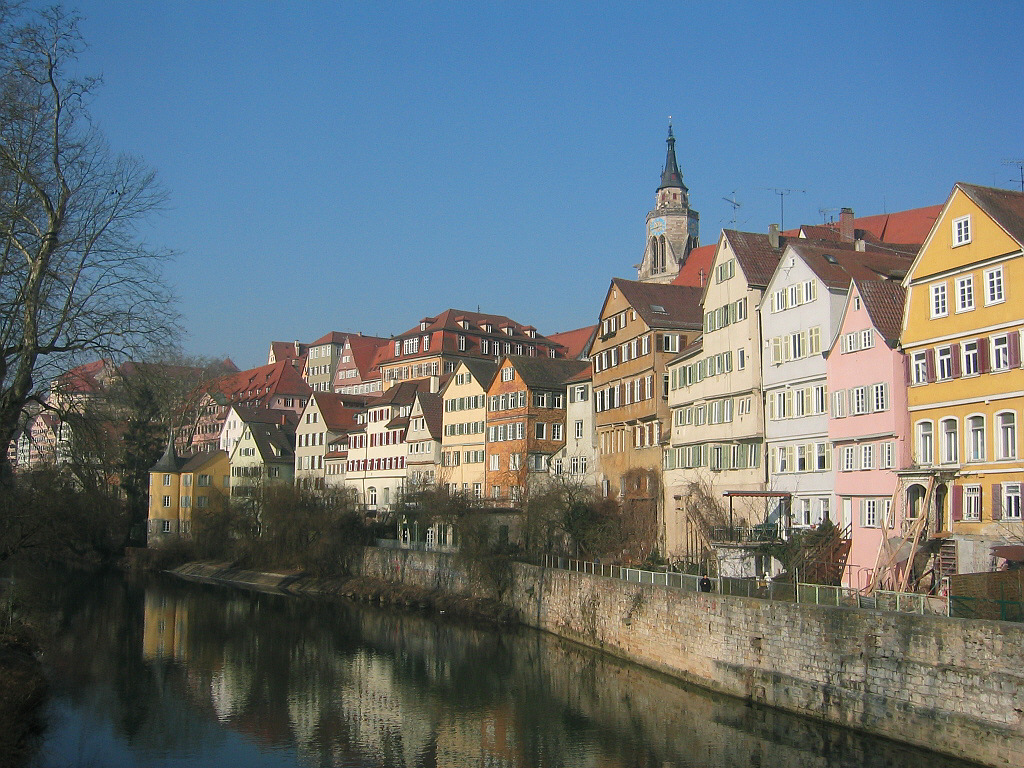
\includegraphics[width=1\textwidth]{neural_style_transfer/img/content/05.jpg} \\
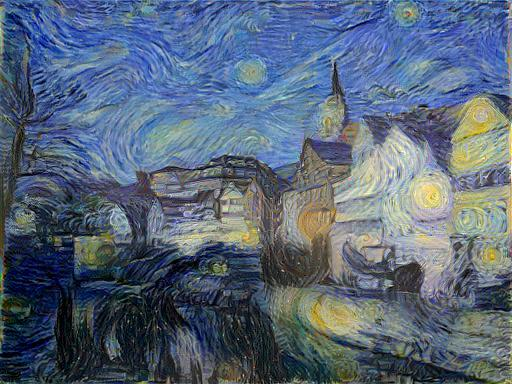
\includegraphics[width=1\textwidth]{neural_style_transfer/img/color_preserve/ret_regu.jpg}
\end{minipage}
}
\subfigure{
\begin{minipage}[b]{0.4\textwidth}
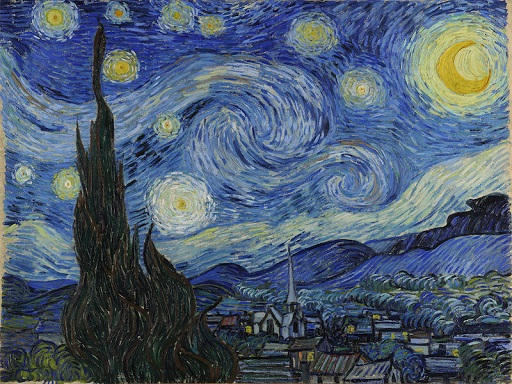
\includegraphics[width=1\textwidth]{neural_style_transfer/img/styles/starry-night.jpg} \\
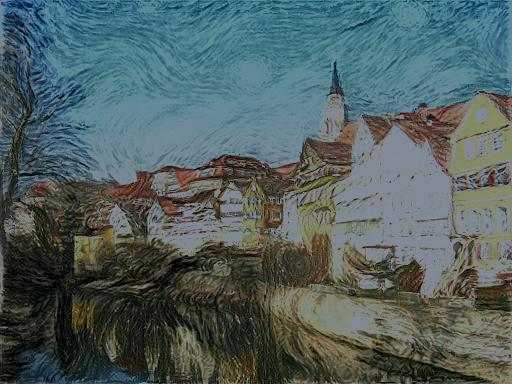
\includegraphics[width=1\textwidth]{neural_style_transfer/img/color_preserve/ret_yuv.jpg}
\end{minipage}
}
\caption{Color-preserving Style Transfer: The top-left image is the content image; the top-right image is the style image; the bottom-left image is the ordinary neural style transfer output; and the bottom-right image is the color preserving transfer output.}
\label{fig:preserve}
\end{figure}


\subsection{Total Variation Regularization}
In Fig.\ref{TV and lap} we compare the performance of the ordinary neural style transfer and the neural style transfer with total variation regularization. The total variation regularization works as a denoising tool, which can smooth the output image. However, in our cases the noise in content image do not have much influence on the quality of final output. Thus, it shows very little difference in Fig.\ref{TV and lap} between the output with and without total variation regularization. The distortion problem in output image will be better solved by the Laplacian-Steered Neural Style Transfer method discussed below.
\begin{figure}[h!]
\centering
\subfigure[Without total variation]{
\begin{minipage}[b]{0.4\textwidth}
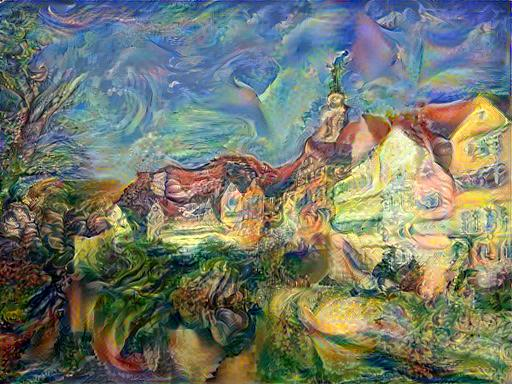
\includegraphics[width=1\textwidth]{neural_style_transfer/img/TV_laplacian/original_output.jpg} \\%original
% 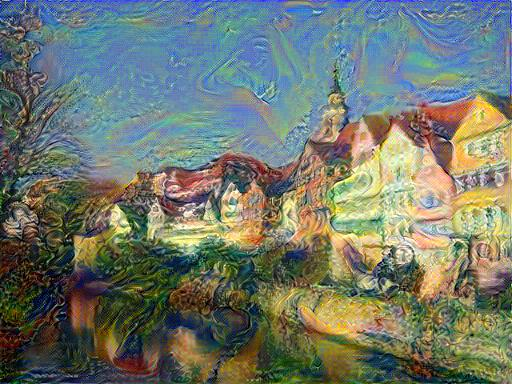
\includegraphics[width=1\textwidth]{neural_style_transfer/img/TV_laplacian/original_output_lap.jpg}%laplace
\end{minipage}
}
% \subfigure[Laplace]{
% \begin{minipage}[b]{0.2\textwidth}
% 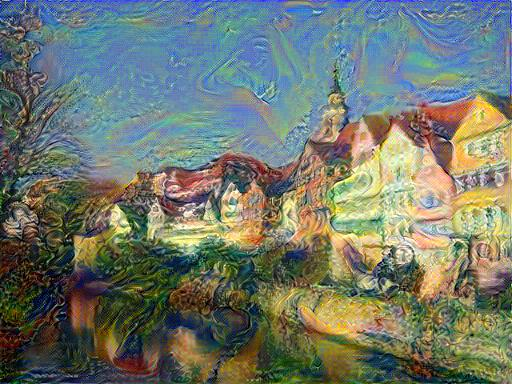
\includegraphics[width=1\textwidth]{neural_style_transfer/img/TV_laplacian/original_output_lap.jpg} \\
% \end{minipage}
% }
\subfigure[Total variation]{
\begin{minipage}[b]{0.4\textwidth}
% 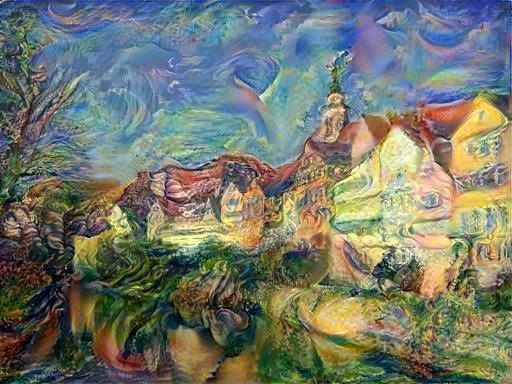
\includegraphics[width=1\textwidth]{neural_style_transfer/img/TV_laplacian/original_output_tv.jpg} \\%TV
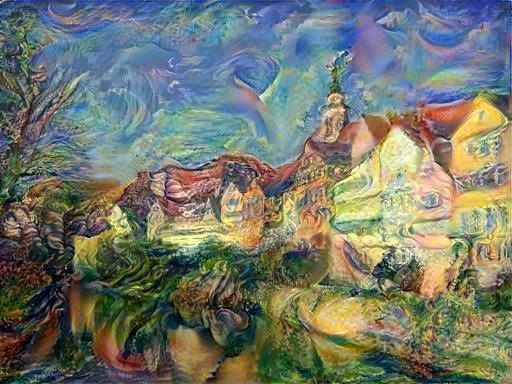
\includegraphics[width=1\textwidth]{neural_style_transfer/img/TV_laplacian/original_output_tv.jpg} \\
\end{minipage}
}
% \subfigure[Total variation and Laplace]{
% \begin{minipage}[b]{0.2\textwidth}
% 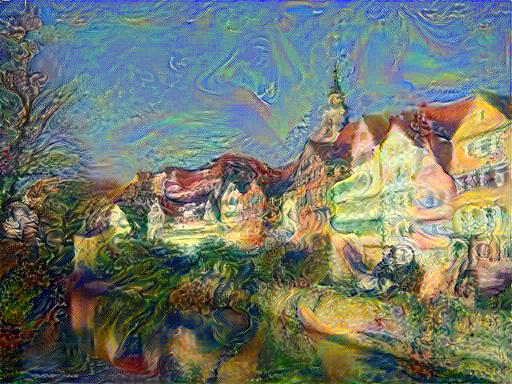
\includegraphics[width=1\textwidth]{neural_style_transfer/img/TV_laplacian/original_output_lap_tv.jpg} \\
% \end{minipage}
% }
\caption{Comparison of neural style transfer with and without total variation regularization}
\label{TV and lap}
\end{figure}

\subsection{Laplacian-Steered Neural Style Transfer}

From Fig.\ref{lap_gamma} we can note from the comparison between the total loss without Laplacian term, e.g. \ref{lap_gamma}(a) and Laplacian loss added in the total loss function, e.g. \ref{lap_gamma}(e), some basic shapes in the building of the content image are preserved in the generated image. Besides, We can see some slight differences  with the different Laplacian loss weights $\gamma$ from Fig.\ref{lap_gamma}(b)-(e), nevertheless reducing $\gamma$ will not change the generated image in a significant way\cite{LiChuan2016CMRF}.


\begin{figure}[h!]
\centering
\subfigure[Without Laplace]{
\begin{minipage}[b]{0.15\textwidth}
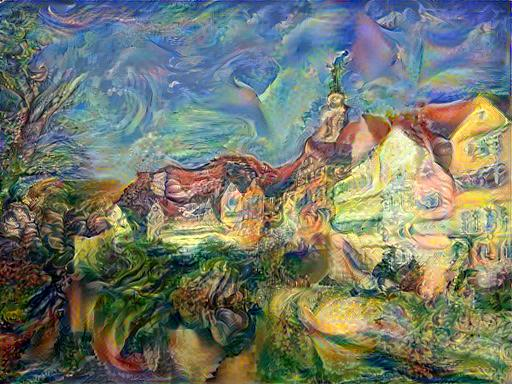
\includegraphics[width=1.1\textwidth]{neural_style_transfer/img/TV_laplacian/original_output.jpg} \\
\end{minipage}
}
\subfigure[$\gamma$=0.1]{
\begin{minipage}[b]{0.15\textwidth}
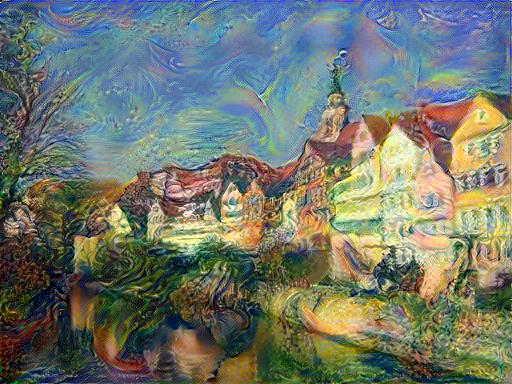
\includegraphics[width=1.1\textwidth]{neural_style_transfer/img/TV_laplacian/original_output_lap-0-1.jpg} \\
\end{minipage}
}
\subfigure[$\gamma$=1]{
\begin{minipage}[b]{0.15\textwidth}
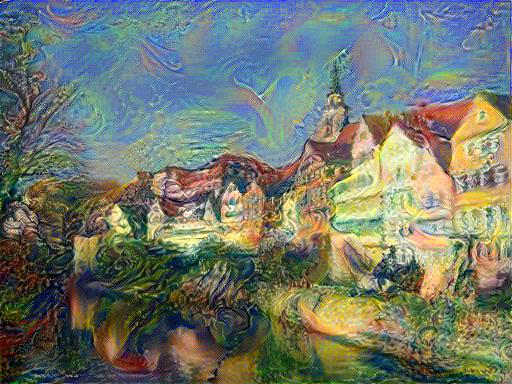
\includegraphics[width=1.1\textwidth]{neural_style_transfer/img/TV_laplacian/original_output_lap-1.jpg} \\
\end{minipage}
}
\subfigure[$\gamma$=10]{
\begin{minipage}[b]{0.15\textwidth}
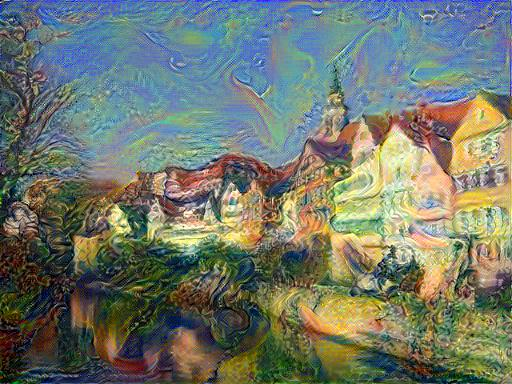
\includegraphics[width=1.1\textwidth]{neural_style_transfer/img/TV_laplacian/original_output_lap-10.jpg} \\
\end{minipage}
}
\subfigure[$\gamma$=150]{
\begin{minipage}[b]{0.15\textwidth}
\includegraphics[width=1.1\textwidth]{neural_style_transfer/img/TV_laplacian/original_output_lap-150.jpg} \\
\end{minipage}
}
\caption{Laplace-Steered Neural Style Transfer with different parameter $\gamma$ setting}
\label{lap_gamma}
\end{figure}

As we mentioned in the method part, the size of pooling layer $p$ have an influence on the quality of the image. A larger size filter will capture the low-level structures in a larger scale, thus multiple Laplacians might have a better result. As we can see in the Fig.\ref{fig:lap_size}, the generated image on the basis of $p=4$ Fig.\ref{fig:lap_size}(b) preserve most of the local structures, while Fig.\ref{fig:lap_size}(c) did not succeed in this due to the size of filter too large. The combination Fig.\ref{fig:lap_size}(d) not only preserve the detailed structures of the content image, but also achieve the best stylization.  
\begin{figure}[h!]
\centering 
\subfigure[Original]{\label{fig:subfig:a}
\includegraphics[width=0.45\linewidth]{neural_style_transfer/img/TV_laplacian/fu2_05_origin.jpg}}
\hspace{0.01\linewidth}
\subfigure[$p=4$]{\label{fig:subfig:b}
\includegraphics[width=0.45\linewidth]{neural_style_transfer/img/TV_laplacian/fu2_05_lap_4-50.jpg}}
\vfill
\subfigure[$p=16$]{\label{fig:subfig:a}
\includegraphics[width=0.45\linewidth]{neural_style_transfer/img/TV_laplacian/fu2_05_lap_16-50.jpg}}
\hspace{0.01\linewidth}
\subfigure[$p_1=4, p_2=16$]{\label{fig:subfig:b}
\includegraphics[width=0.45\linewidth]{neural_style_transfer/img/TV_laplacian/fu2_05_lap_4-16-50-50.jpg}}
\caption{Comparison of Laplacian with difference pooling sizes}
\label{fig:lap_size}
\end{figure}


\section{Conclusions}
In this project, we first replicate Gatys \textit{et al.}'s work to realize the neural style transfer system. We find out that by changing the content/style ratio in the loss function, as well as using different layers of the VGG-19 network, we can get different output image.

Secondly, we realize some further functions based on the original theory of neural style transfer. The multi-style transfer can synthesis an image with content from one image, and style from two or more other images. By changing the weights before the loss of the style images, we can get the output we like. The color-preserving transfer can help the output image get rid of the influence of style image on its color. By using the method of luminance-only transfer, we realize this function ideally.

Moreover, we improve the loss function by adding a total variation regularization term onto it. This term can denoise the content image, and make the output image more smooth. However, the output image does not change much after this altering.

Finally, we add a Laplacian term to the loss function to get rid of some distortions and irregular artifacts in the output image. Our results show that this method can help maintain the pixel level information while remaining the transferred style. Also, according to the experiments we suppose that transfer results may depend on the initial content image or style image somehow.

% \newpage
% \section{Appendix}
% \begin{table}[h!]
% \begin{center}
% \caption{The Structure of VGG-19 Network}
% \label{table:VGG}
% \begin{tabular}{|c |c | c |c|}
% \hline
%      & \textbf{Layer Name} & \textbf{Group No.}  \\
%      \cline{1-3}
%      1 & conv1\_1 & \multirow{Group-1}\\
%      \cline{1-2}
%      2 & relu1\_1 &  \\
%       \cline{1-2}
%      3 & conv1\_2 &  \\
%       \cline{1-2}
%      4 & relu1\_2 &  \\
%       \cline{1-2}
%      5 & pool1 &  \\
%      \cline{1-3}
%      6 & conv2\_1 & \multirow{Group-2}\\
%      \cline{1-2}
%      7 & relu2\_1 &  \\
%       \cline{1-2}
%      8 & conv2\_2 &  \\
%       \cline{1-2}
%      9 & relu2\_2 &  \\
%       \cline{1-2}
%      10 & pool2 &  \\
%      \cline{1-3}
%      11 & conv3\_1 & \multirow{Group-3}\\
%      \cline{1-2}
%      12 & relu3\_1 &  \\
%       \cline{1-2}
%      13 & conv3\_2 &  \\
%       \cline{1-2}
%      14 & relu3\_2 &  \\
%       \cline{1-2}
%      15 &conv3\_3 &  \\
%      \cline{1-2}
%      16 &relu3\_3 &  \\
%      \cline{1-2}
%      17 &conv3\_4 &  \\
%      \cline{1-2}
%      18 &relu3\_4 &  \\
%      \cline{1-2}
%      19 & pool3 & \\
%      \cline{1-3}
%      20 & conv4\_1 & \multirow{Group-4}\\
%      \cline{1-2}
%      21 & relu4\_1 &  \\
%       \cline{1-2}
%      22 & conv4\_2 &  \\
%       \cline{1-2}
%      23 & relu4\_2 &  \\
%       \cline{1-2}
%      24 &conv4\_3 &  \\
%      \cline{1-2}
%      25 &relu4\_3 &  \\
%      \cline{1-2}
%      26 &conv4\_4 &  \\
%      \cline{1-2}
%      27 &relu4\_4 &  \\
%      \cline{1-2}
%      28 &pool4 &  \\
%      \cline{1-3}
%      29 & conv5\_1 & \multirow{Group-5}\\
%      \cline{1-2}
%      30 & relu5\_1 &  \\
%       \cline{1-2}
%      31 & conv5\_2 &  \\
%       \cline{1-2}
%      32 & relu5\_2 &  \\
%       \cline{1-2}
%      33 &conv5\_3 &  \\
%      \cline{1-2}
%      34 &relu5\_3 &  \\
%      \cline{1-2}
%      35 &conv5\_4 &  \\
%      \cline{1-2}
%      36 &relu5\_4 &  \\
%      \cline{1-2}
%      37 &pool5 &  \\
%      \cline{1-3}
% \hline
% \end{tabular}
% \end{center}
% \end{table}

% The paper ends with a conclusion. 


% \clearpage\mbox{}Page \thepage\ of the manuscript.
% \clearpage\mbox{}Page \thepage\ of the manuscript.
% \clearpage\mbox{}Page \thepage\ of the manuscript.
% \clearpage\mbox{}Page \thepage\ of the manuscript.
% \clearpage\mbox{}Page \thepage\ of the manuscript.
% \clearpage\mbox{}Page \thepage\ of the manuscript.
% \clearpage\mbox{}Page \thepage\ of the manuscript.
% This is the last page of the manuscript.
% \par\vfill\par
% Now we have reached the maximum size of the ECCV 2016 submission (excluding references).
% References should start immediately after the main text, but can continue on p.15 if needed.

\clearpage

\bibliographystyle{splncs}
\bibliography{egbib}
% \bibliography{Review-Cheng}Jing, Y. et al., 2017. Neural Style Transfer: A Review.
\end{document}
